\documentclass{article}


% if you need to pass options to natbib, use, e.g.:
% \PassOptionsToPackage{numbers, compress}{natbib}
% before loading nips_2018

% ready for submission
\usepackage{nips_2018}

% to compile a preprint version, e.g., for submission to arXiv, add
% add the [preprint] option:
%\usepackage[preprint]{nips_2018}

% to compile a camera-ready version, add the [final] option, e.g.:
%\usepackage[final]{nips_2018}

% to avoid loading the natbib package, add option nonatbib:
% \usepackage[nonatbib]{nips_2018}

\usepackage[utf8]{inputenc} % allow utf-8 input
\usepackage[T1]{fontenc}    % use 8-bit T1 fonts
\usepackage{hyperref}       % hyperlinks
\usepackage{url}            % simple URL typesetting
\usepackage{booktabs}       % professional-quality tables
\usepackage{amsfonts}       % blackboard math symbols
\usepackage{nicefrac}       % compact symbols for 1/2, etc.
\usepackage{microtype}      % microtypography
\usepackage{textcomp}
\usepackage{amsmath}
\usepackage{graphicx}
\usepackage{multirow}
\usepackage{multicol,color}

\title{Secure Computation for Machine Learning With SPDZ}

% The \author macro works with any number of authors. There are two
% commands used to separate the names and addresses of multiple
% authors: \And and \AND.
%
% Using \And between authors leaves it to LaTeX to determine where to
% break the lines. Using \AND forces a line break at that point. So,
% if LaTeX puts 3 of 4 authors names on the first line, and the last
% on the second line, try using \AND instead of \And before the third
% author name.

\author{
  Valerie Chen\\
  Yale University\\
  %% Address?? \\
  \texttt{v.chen@yale.edu} \\
  \And
  Valerio Pastro\\
  Yale University\\
  \texttt{valerio.pastro@yale.edu}\\
  %% examples of more authors
  \And
  Mariana Raykova \\
  Yale University \\
  %% Address?? \\
  \texttt{mariana.raykova@yale.edu} \\
  %% \AND
  %% Coauthor \\
  %% Affiliation \\
  %% Address \\
  %% \texttt{email} \\
  %% \And
  %% Coauthor \\
  %% Affiliation \\
  %% Address \\
  %% \texttt{email} \\
  %% \And
  %% Coauthor \\
  %% Affiliation \\
  %% Address \\
  %% \texttt{email} \\
}

\begin{document}

\maketitle

\begin{abstract}
Secure Multi-Party Computation (MPC) is an area of cryptography, which enables the computation on sensitive data from multiple sources while maintaining privacy guarantees.
However, theoretical protocols often do not scalable efficiently to real world size data. This project investigates the efficiency of of the SPDZ framework~\cite{SPDZ12}, which provides implementation
of MPC protocols with malicious security, in the context of popular machine learning (ML) algorithms. In particular, we choose applications such as linear regression and logistic regression,
which have been implemented and evaluated using semi-honest MPC techniques~\cite{GSB0DZE17, MZ17}. We demonstrate that the SPDZ framework outperforms these previous implementations while providing stronger security.
\end{abstract}


\section{Introduction}

Many machine learning techniques, including regression analysis, aim to build a model that fits a set of predictors to a dependent variable. Such techniques are widely used to model and analyze big data.
In many settings, however, the input data for such ML analysis tools is partitioned among different parties, which have strict privacy policies. For example, the Center for Disease Control is interested in identifying disease outbreak and many individual hospitals have their own patients' data which could benefit this study. The problem is that openly sharing this data for prediction or model-building purposes would be against modern day privacy laws as it would leak private individual data. This is one of many examples, which could benefit of the functionality that allows to evaluate to output of the analysis without revealing more about the private inputs.
%This application of secure MPC is one that would be extremely valuable in today\textquotesingle s world.

\subsection{Multi-Party Computation}

Secure MPC addresses the above problem by providing a mechanism through which different parties can run a joint computation over their private inputs with guarantees that the only thing
revealed about the inputs, is the output of the computation and whatever can be inherently inferred from it.
There are two main types of MPC protocols in terms of their security guarantees: semi-honest and malicious protocols \cite{Goldreich:2004:FCV:975541, cryptoeprint:2010:551}. In semi-honest security, it is assumed that the parties will follow the protocol as specified, but they can try to infer information about the input from the protocol messages. In malicious security, dishonest parties may attempt to deviate from the specified protocol, and the protocol must guarantee that these parties cannot learn about the inputs. Since malicious protocols have to satisfy stronger guarantees in general such construction are less efficient than semi-honest protocols.

Two recent works~\cite{GSB0DZE17, MZ17} propose efficient implementation for several central building blocks for machine learning such as conjugate gradient decent (CGD) and stochastic gradient descent (SGD) as well as applications  using them such as linear and logistic regression.  The work of Gascon et al.~\cite{GSB0DZE17} uses the framework for semi-honest computation Obliv-C~\cite{cryptoeprint:2015:1153} and proposes
several different methods for solving systems of linear equations. Their main premise is to use an iterative method such as CGD and show trade-offs that save a lot of computation and hence efficiency for the MPC in
return for a small accuracy loss. They further propose a modification of CGD that has stable behavior using fix-point arithmetic since emulating floating point with the underlying MPC representation introduces substantial
efficiency overhead.

The work of Mohassel and Zhang~\cite{MZ17} considers stochastic gradient descent as a method for learning linear regression and logistic regression by using different activation functions. The authors consider
arithmetic representation for the computation and propose new secure computation techniques for matrix computation, which generalize the approach for generating multiplicative triples in a preprocessing step.
 Similarly to the work of Gascon et al.~\cite{GSB0DZE17}, this paper considers techniques for approximation that save computation, for example, using a piece-wise approximation for the logistic function. The author
 also propose new techniques for more efficient approximate computation of fixed-point encodings.

The techniques in both of the above works are restricted to the setting of two party computation. We choose the SPDZ~\cite{SPDZ12,KSS13,KPR18} framework for our implementations since it is one of the main and most comprehensive 
implementations for multiparty computation protocols, which provide malicious security and support more than two parties.

\iffalse
For this study, we chose the SPDZ framework [1,6], which ensures against malicious security, and compare against two semi-honest methods Obliv-C [10] and SecureML [8]. The SPDZ protocol is comprised of an efficient preprocessing offline phase using semi-homomorphic encryption and an optimized secret-sharing online phase that computes an arithmetic circuit. Obliv-C is based on Yao\textquotesingle s garbled circuits and Gascon et al.[4]  introduces optimizations on inner products and algorithmic modifications to speed up regression calculation. SecureML developed MPC-friendly alternatives to non-linear activation functions which are often intensive to compute as well as vectorization techniques in a shared setting. 

Secure computation is slower and could have lower accuracy when compared to the same computation in plaintext. Thus trade-offs need to be made in terms of the accuracy and the complexity of the algorithm, which will affect the MPC efficiency.
\fi


\section{ML Functionalities}

%Our goal was to evaluate and compare the performance of SPDZ against other frameworks in the context of ML applications that have been previously considered in [4,8], evaluating in terms of runtime and accuracy. 
For our implementation we consider the same algorithms and functionalities as in the above two papers. Next we provide a brief overview of these classic algorithms (details can be found in ~\cite{HTF09}).

%The main algorithms that we considered were: LDLT Decomposition, Cholesky, Conjugate Gradient Descent (CGD), Stochastic Gradient Descent (SGD), Logistic Regression. These are classic algorithms that can be found in standard machine textbooks (e.g., [3]). 

%In our evaluation, the algorithms were implemented in the SPDZ framework as well as in python as a plaintext verification of the algorithm.

\subsection{Direct vs. Iterative Decomposition for Solving a Linear System}

Solving a system of linear equations, which underlies linear regression learning, can be done using techniques for direct and indirect decomposition.
LDLT and Cholesky are both variants of direct decomposition methods which decompose a Hermitian, positive-definite matrix into a lower triangular matrix and its conjugate transpose. The algorithms are cubic in complexity with asymptotic run time of $O(d^3)$, where $d$ is the dimension of the input matrix. 
%This runtime can become inefficient when considering real world data that have large number of features and entries. 
The difference between LDLT and Cholesky is that Cholesky requires a square root. The representation of square root computation as an arithmetic circuit used in the MPC computation in SPDZ introduces 
considerable overhear. That is why we used the iterative Newton method as a way of approximating the square root computation. It computes $x_i$, where $x_{i}^2 = S$, with repetition of the following
update function $x_{n+1} =1/2 (x_{n} + S/x_{n})$.

\iffalse
In MPC, non-linear functions like square roots are difficult to represent due to the linear nature of secret sharing schemes. Thus, we looked at an iterative Newton method as a way of approximating the square root in SPDZ to solve for $x_i$, where $x_{i}^2 = S$:

\[
x_{n+1} = \frac{1}{2} (x_{n} + \frac{S}{x_{n}})
\]
\fi

In terms of an iterative approach to regression, we used the approach proposed by
Gascon et al.~\cite{GSB0DZE17}, which uses a normalized version of CGD that preserves stability and convergence rate with fixed-point number representation. Similarly to other MPC implementations
using floating point representation in SPDZ introduces substantial efficiency overhead. 

%proposed a modification for the normalization in the iterative version of CGD that would be more stable with fixed-point numbers. We applied the same algorithm to SPDZ to see if the same modification would work. The goal of comparing iterative versus a direct method would be to justify the potential accuracy trade off for a much smaller run time.

\subsection{Stochastic Gradient Descent}

Stochastic gradient descent is an iterative approximation method that converges to the global minimum for convex problems, like linear and logistic regression. It is also a driving mechanism for non-convex problems like neural networks. An SGD iteration updates a weight vector $\mathbf{w}$ using a randomly selected sample from the training input as follows: $w_j := w_j - \alpha ({\partial C_i(\mathbf{w})}/{\partial w_j})$ with learning rate $\alpha$. In this update $C_i$ is the cost function, which can be instantiated with different concrete functions to obtain computation for linear regression and logistic regression. A common technique for SGD
computation is called \emph{mini-batch} -- instead of selecting one sample per iteration, a small batch of size $B$ samples are selected and the update function is performed averaging the partial derivatives across all samples. We use the mini-batch SGD in our implementation to obtain accuracy benefits. While the work of Mohassel and Zhang~\cite{MZ17} has optimizations for matrix computation, which can be used with mini-batch, for 
SPDZ this does not lead to additional savings.
 

\iffalse
In a linear regression setting, we update the learned weights $w$, given learning rate $\alpha$ and input matrix $x$ and expected output $y$, using $w_j = w_j  - \alpha(x_i \cdot w *-y_i)x_{ij}$ [8]. In this update function, the weights are adjusted element-wise by the error from the predicted and expected value at a rate determined by $\alpha$.

Instead of selecting one sample per iteration, a small batch of size $B$ samples are selected and the update function is performed collectively. We implemented this modification called mini-batch SGD so the weights would converge more quickly and in smoother fashion to the minimum. Since SPDZ does not support vectorization (e.g. in python), where operations are broadcasted to entire array, we were not able to take advantage of the time speed-ups. However we were still able to take advantage of the accuracy benefit. The algorithm for the batched version is modified as such, where $w$ are the weights, $\alpha$ the learning rate, $X_{B}$ the batched input, and $Y_{B}$ the corresponding expected batched output: 
\[
 w = w - \frac{1}{|B|} \alpha X^{T}_{B} \times (X_{B} \times w - Y_{B})
\]
\fi

\subsubsection{Linear and Non-Linear Activation Functions}

To obtain a solution for linear regression using SGD, we instantiate the cost function as $w_j = w_j  - \alpha(X_i \cdot w *-y_i)X_{ij}$, where $X$ is the input matrix and $y$ is the input vector. In this update function, the weights are adjusted element-wise by the error from the predicted and expected value at a rate determined by $\alpha$.

Logistic regression is a classification algorithm for modeling a binary dependent variable. Logistic regression fits the logistic function $f(u) = \frac{1}{1+e^-u}$ to the input. The corresponding update function for mini-batched SGD for logistic regression is $ w = w - \frac{1}{|B|} \alpha X^{T}_{B} \times f(X_{B} \times w - Y_{B})$, where $f$ maps the predicted value into the binary output space. Mohassel and Zhang [8] proposed the following piecewise function as approximation for $f$:

\[
  f(u) =
  \begin{cases}
                                   0 & \text{if $u < -0.5$} \\
                                   u + 0.5 & \text{if $-0.5 \leq u \leq 0.5$} \\
1 & \text{if $u > 0.5$}
  \end{cases}
\]

We compare the results of this MPC-friendly piecewise function to a more standard approximation approach of taking the Taylor Series expansion to varying degrees.

\section{Experiments}

\subsection{Experimental Setup}

For our evaluation, we implemented all algorithms both in the SPDZ framework as well as in python as a plaintext verification of the algorithm.
The main metrics of evaluations were the latency of the MPC computation and the accuracy error, and we aimed to explore the trade-offs between accuracy and efficiency. We varied the precision after the decimal point 
depending on what was used in the works that we compared against (32 and 64 bits for the linear regression, less for SGD).

We evaluated our methods on both real-world datasets (MNIST, Arcene, and 9 other UCI open-source datasets) as well as synthetically generated data. These real-world datasets allow us to compare the accuracy results to existing works and to demonstrate that SPDZ can be used in practical settings. We used synthetic data in order to explore larger ranges of data characteristics such as dimension ($d$ = 10, 20, 50, 100, 200, 500), condition number ($cd$ = [1,10]), and number of examples ($n$ = 1000, 100000).

Most of our experiments were ran using machines on the same local area network where there is no network latency. We performed tests where both parties were deployed on separate Amazon EC2 m4.large instances.
We also ran experiment with up to four parties.

%In our experiments, both parties were mostly run on one machine to simplify the procedure, but we also performed tests where both parties were deployed on separate Amazon EC2 m4.large instances. It is important to note that the distribution of players across machine only affects runtime and not the accuracy of the results. We also looked at up to four parties as a form of validation of the SPDZ protocol.

\subsection{Results}

In this section we present empirical results for our SPDZ implementations evaluated with real and synthetic databases. We compare the five different algorithms in terms of accuracy and run time for various parameters. 

\begin{figure}[h!]
\centering
  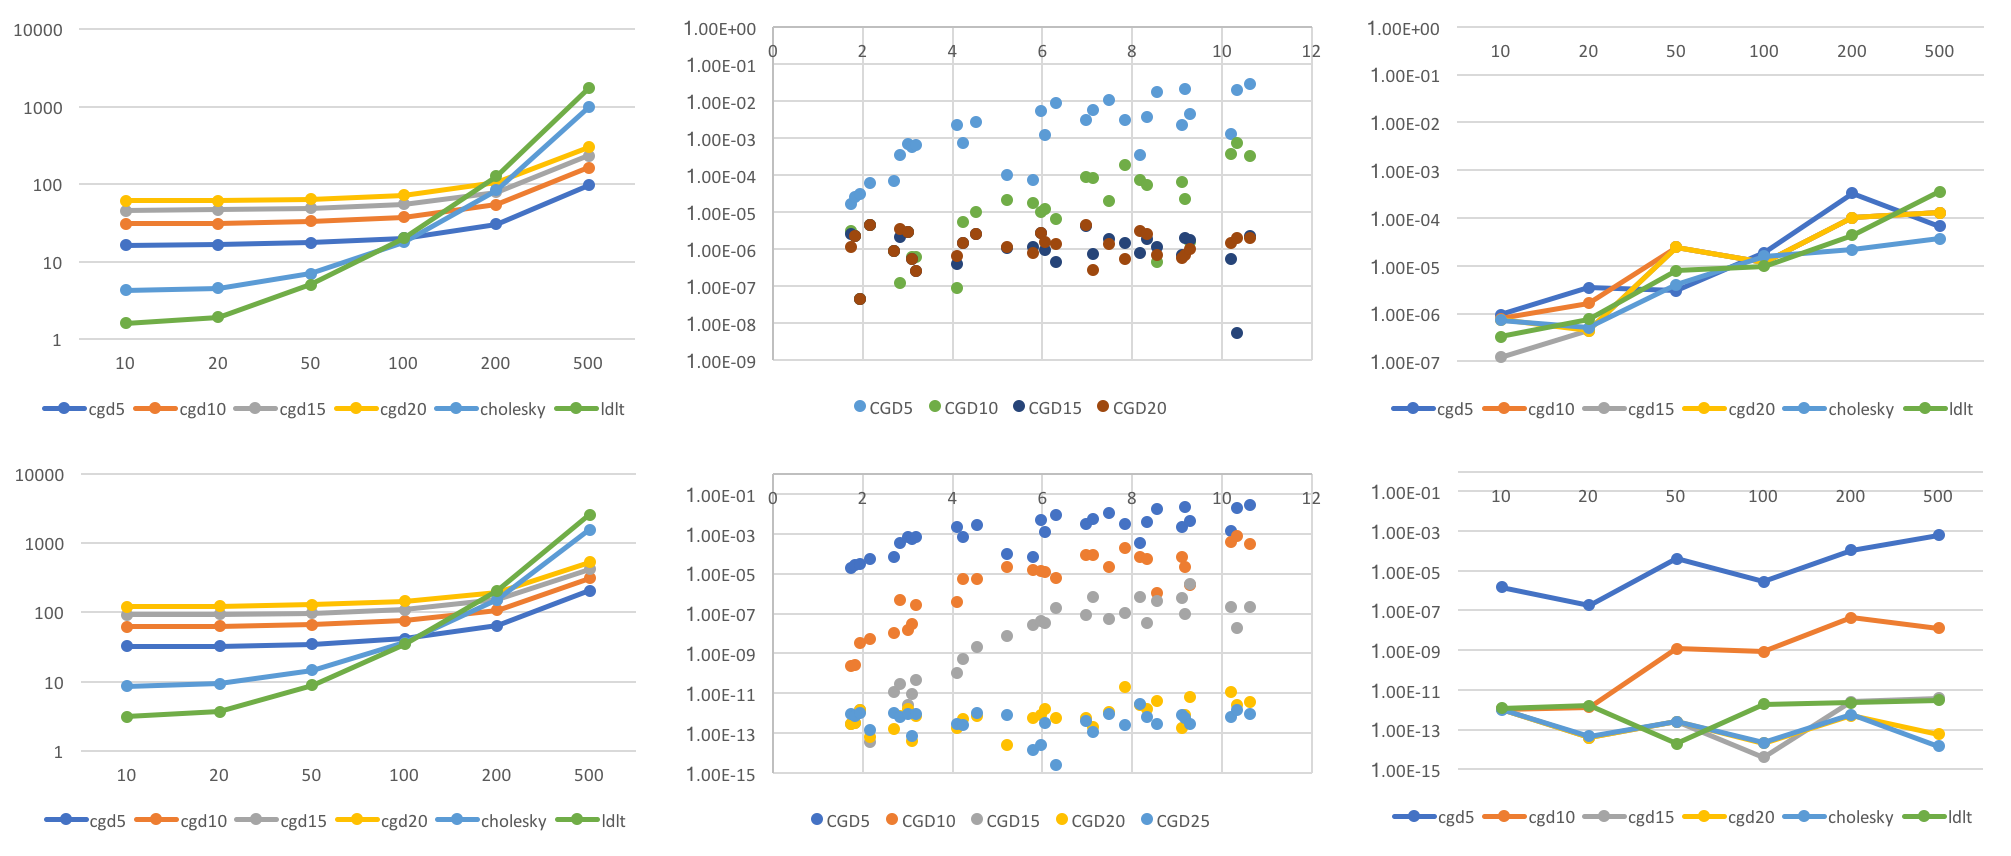
\includegraphics[scale=0.4]{allregression.png}
    \caption{(Left) Run time as a function of input dimension. (Middle) Condition number as a function of accuracy. (Right) Accuracy as a function of the input dimension. (Top) Fixed-point with 60 bits of precision. (Bottom) Fixed-point with 28 bits of precision}
   \label{fig:result1}   
\end{figure}

For LDLT, Cholesky and various iterations of CGD, we evaluated on synthetically generated data of varying sizes and condition numbers. The larger the condition number is, the larger the error in approximations of the solution is. The direct decomposition methods grew exponentially in run time as input size increases, which is shown in the left column of Figure~\ref{fig:result1} -- this unlikely to be suitable for large size real data. Alternatively, the iterative CGD runtime increases at a much slower rate. In the middle column of Figure 2, we find that about 20 iterations are sufficient to reach maximum accuracy given the number of allocated bits even with varying condition numbers. Particularly for the 64-bit case, shown on the bottom right, the accuracy is identical for CGD after 15 iterations and Cholesky/LDLT.

\begin{figure}[h!]
\vspace{-4mm}
\centering
  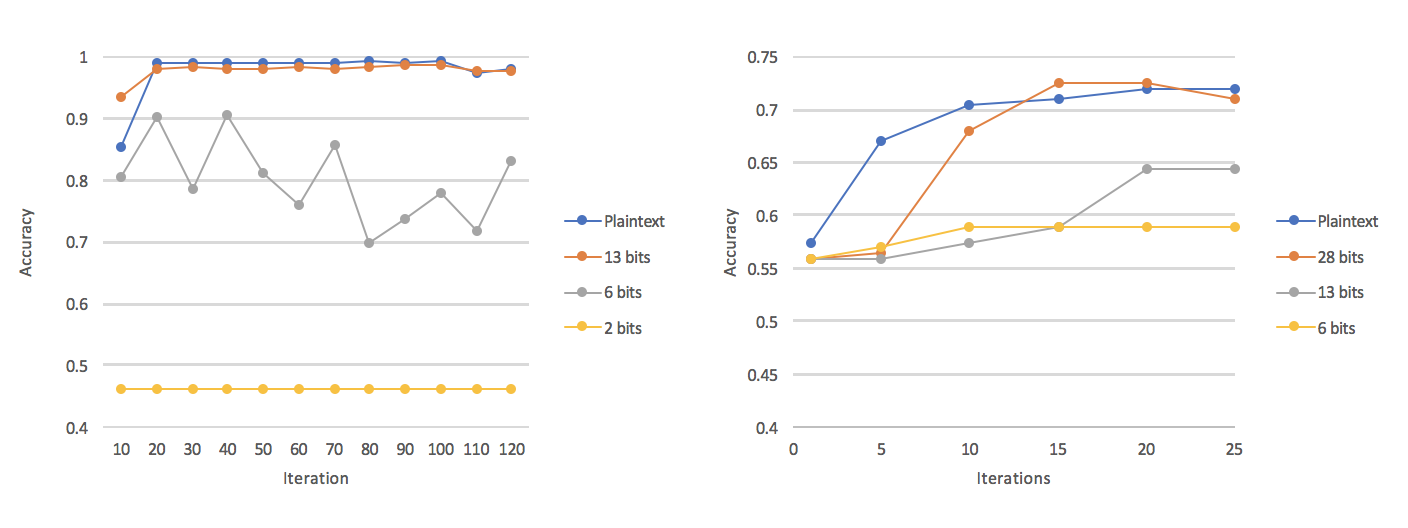
\includegraphics[scale=0.6]{mnistarcene.png}
  \vspace{-4mm}
   \caption{Comparing accuracy of privacy preserving linear regression with various fixed point precisions and plaintext training on floating point for MNIST (left) and Arcene (right).}
   %\vspace{-4mm}
   \label{fig:result2}  
\end{figure}

Figure~\ref{fig:result2} compares SGD on MNIST and Arcene results. It shows that the number of bits of precision needed to get good accuracy is highly dependent on the dataset. For MNIST, 13 bits was sufficient to match plaintext accuracy but 28 bits were needed for Arcene. The MNIST data contains only 784 features while there are 10,000 in the Arcene data, 3,000 of which are considered "probes" with no predictive power, which could explain the lower overall accuracy of \cite{MZ17}. While the numbers in the MNIST data ranged from 0 to 9, Mohassel and Zhang~\cite{MZ17} only used 0s and 1s labels from the dataset, reducing it to a binary problem. We replicated this approach and present the results below. We did run the computation to predict all 10 digits, but found that SGD only achieved a much lower accuracy of about 19\%. We also compared the root mean squared error (RMSE) of SGD on 9 UCI open-sourced datasets of ranging sizes to results in \cite{GSB0DZE17}. Our results in the SPDZ secure setting typically increased RMSE by about $5-20\%$ compared to plaintext computation, but still outperformed RMSE results from \cite{GSB0DZE17} in both CGD and SGD.

In terms of logistic regression, for SPDZ, we did not find that the new activation function was a better alternative to taking a Taylor Series approximation for the exponential function as shown in Table~\ref{tbl1}. We found that for SPDZ, which is based on arithmetic circuits, the extra time to take a few extra degrees in the approximation was negligible.  

\begin{table}[h!] 
\caption{Comparing the validation accuracy for different activation functions for logistic regression.}
\centering
\label{my-label}
\begin{tabular}{@{}lllllll@{}}
\toprule
       & Plaintext & New Activation function & \multicolumn{4}{l}{Polynomial Approximation} \\
       &           &                         & degree 2  & degree 5  & degree 7 & degree 10 \\ \midrule
MNIST  & 99.9\%    & 95\%                    & 97\%      & 85\%      & 91\%     & 99.5\%    \\
Arcene & 72.0\%    &           44.0\%              &   44.0\%        &    44.5\%       &    65\%      &    72\%       \\ \bottomrule
\end{tabular}
\vspace{-4mm}
\label{tbl1}
\end{table}

\subsection{Conclusion}

We found that the SPDZ outperformed Obliv-C even in a distributed machine setting by an order of magnitude and achieves comparable results to SecureML for SGD instantiations such as Linear and Logistic Regression. The accuracy findings were comparable for LDLT, Cholesky, and CGD results for SPDZ and Obliv-C, but we found that SPDZ outperformed Obliv-C on SGD. SPDZ was able to match SecureML results on SGD and Logistic Regression.

%\section*{References}

\bibliographystyle{plain}
\bibliography{refs}

\iffalse

\small

[1] Damg\aa rd, I., Keller, M., Larraia, E., Pastro, V., Scholl, P., \& Smart, N. P. (2013). Practical covertly secure MPC for dishonest majority?or: breaking the SPDZ limits. {\it European Symposium on Research in Computer Security}, pp.\ 1-18.

[2] Du, W., \& Atallah, M. J. (2001). Secure multi-party computation problems and their applications: a review and open problems. {\it Proceedings of the 2001 workshop on New security paradigms}, pp.\ 13-22. ACM.

[3] Friedman, J., Hastie, T., \& Tibshirani, R. (2001). The elements of statistical learning (Vol. 1, No. 10). New York, NY, USA:: Springer series in statistics.

[4] Gasc\'{o}n, A., Schoppmann, P., Balle, B., Raykova, M., Doerner, J., Zahur, S., \& Evans, D. (2017). Privacy-preserving distributed linear regression on high-dimensional data. {\it Proceedings on Privacy Enhancing Technologies, 2017(4)}, pp.\ 345-364.

[5] Hazay, C., \& Lindell, Y. (2010). A Note on the Relation between the Definitions of Security for Semi-Honest and Malicious Adversaries. {\it IACR Cryptology ePrint Archive}, pp.\ 551.

[6] Keller, M., Scholl, P., \& Smart, N. P. (2013). An architecture for practical actively secure MPC with dishonest majority. {\it Proceedings of the 2013 ACM SIGSAC conference on Computer \& communications security}, pp.\ 549-560. ACM.

[7] Lindell, Y., \& Pinkas, B. (2009). A proof of security of Yao?s protocol for two-party computation. Journal of Cryptology, 22(2), 161-188.

[8] Mohassel, P., \& Zhang, Y. (2017). SecureML: A system for scalable privacy-preserving machine learning. {\it 38th IEEE Symposium on Security and Privacy (SP)}, pp. 19-38. IEEE.

[9] Phung, D., Tseng, V. S., Webb, G. I., Ho, B., Ganji, M., \& Rashidi, L. (Eds.). (2018). Advances in Knowledge Discovery and Data Mining: 22nd Pacific-Asia Conference, PAKDD 2018, Melbourne, VIC, Australia, June 3-6, 2018, Proceedings (Vol. 10938). Springer.

[10] Zahur, S., \& Evans, D. (2015). Obliv-C: A Language for Extensible Data-Oblivious Computation. {\it IACR Cryptology ePrint Archive, 2015}, 1153.

\fi

\end{document}


%Can add table back in - I am describing results instead. 
%\begin{table}[h!]
%\caption{Runtime results against }
%\centering
%\begin{tabular}{@{}llcl@{}}
%\toprule
%\multicolumn{1}{c}{Datasets}                                           & \multicolumn{3}{c}{Runtime (seconds)}                                      \\ \midrule
%CGD (64 bit)                                                           & \multicolumn{1}{c}{Ours} & Ours (EC2) & \multicolumn{1}{c}{Obliv-C}        \\ \midrule
%d=100                                                                  & 144                      & 243        & \textgreater $10^3$ \\ \midrule
%d=500                                                                  & 527                      & 2701       & \textgreater $10^4$ \\ \midrule
%\multirow{2}{*}{\begin{tabular}[c]{@{}l@{}}SGD: \\ MNIST\end{tabular}} & \multicolumn{1}{c}{Ours} & \multicolumn{2}{c}{SecureML}                    \\ \cmidrule(l){2-4} 
%                                                                       & 10200                    & \multicolumn{2}{c}{10330}                       \\ \bottomrule
%\end{tabular}
%\end{table}

%\section{Conclusion}

%Through this work, we demonstrated that SPDZ, a malicious security framework, can match the efficiency and accuracy other protocols of semi-honest through experiments on real and synthetic data. This investigation into the applicability of secure MPC on real world data demonstrates its potential change the way data is used in a variety of applications in today\textquotesingle s world.
